\documentclass[11pt]{article}
\usepackage{times}
\newif\ifpdf
\ifx\pdfoutput\undefined
  \pdffalse
  \usepackage[dvips]{graphicx}    
  \usepackage[dvips]{color}  
\else
  \pdftrue
  \usepackage[pdftex]{graphicx}    
  \usepackage[pdftex]{color}  
\fi
\usepackage{fullpage}
\usepackage{url}
\usepackage{cite}
\usepackage{alg}
\bibliographystyle{bmc_bioinformatics}

\def\argmax{\mathop{\mathrm{argmax}}\limits}
\def\argmin{\mathop{\mathrm{argmin}}\limits}

\setcounter{secnumdepth}{0}

\begin{document}

\title{A memory-efficient dynamic programming algorithm for optimal
alignment of a sequence to an RNA secondary structure consensus model}
\author{Sean R. Eddy\\
Howard Hughes Medical Institute \& Department of Genetics, \\
Washington University School of Medicine \\
Saint Louis, Missouri 63110 USA \\
eddy@genetics.wustl.edu}  
\date{\today}
\maketitle

\abstract{Covariance models (CMs) are probabilistic RNA secondary
structure models, analogous to profile hidden Markov models for linear
sequence consensus. The standard CYK algorithm for optimal dynamic
programming alignment of a CM to an RNA sequence is $\Theta(N^3)$ in
memory for an RNA of length $N$. On current computers, this is only
practical for small RNAs of a few hundred nucleotides or less. Here I
describe a divide and conquer variant of the CM/SCFG alignment
algorithm, analogous to the memory-efficient Myers/Miller form of the
Smith/Waterman algorithm for linear sequence alignment. The algorithm
has an average memory requirement that scales as $(N^2 \log N)$, at
the expense of a small constant factor in time. Small subunit
ribosomal RNA alignments that previously required a prohibitive 20-30
GB of memory to solve by dynamic programming now require $\approx$ 80
MB and are well within the capabilities of most modern computers.}

\section{Introduction}

We know of a growing number of RNA gene families and RNA motifs
\cite{Eddy01,Erdmann01}. Many (though not all) RNAs of interest
conserve a base-paired RNA secondary structure. Computational analyses
of RNA sequence families are more powerful if they take into account
both primary sequence and secondary structure consensus.

Some excellent approaches have been developed for database searching
with RNA secondary structure consensus patterns. Exact- and
approximate-match pattern searches (a la PROSITE patterns) have been
extended to allow patterns to specify long-range base pairing
constraints \cite{Laferriere94,Dsouza97}. Another approach involves
developing a specialized program to recognize a specific type of RNA
\cite{Dandekar95} -- for example, programs exist for detecting
transfer RNA genes \cite{Fichant91,El-MabroukLisacek96,LoweEddy97},
group I catalytic introns \cite{Lisacek94}, or small nucleolar RNAs
\cite{Nicoloso96,LoweEddy98}. These approaches, though powerful, lack
generality, and they tend to require expert knowledge about each
particular RNA family of interest.

In primary sequence analysis, a technologically more mature field, the
main techniques are neither pattern searches nor specialized
programs. The main analysis techniques are primary sequence alignment
algorithms with probabilistically-based scoring systems -- for
example, the BLAST \cite{Altschul97}, FASTA \cite{Pearson88}, or
CLUSTALW \cite{Thompson94b} algorithms, and the PAM \cite{Dayhoff78}
or BLOSUM \cite{Henikoff92} score matrices. Unlike specialized
programs, a general alignment algorithm can be applied to any query
sequence(s). Unlike pattern searches, which give yes/no answers for
whether a candidate sequence is a match, a scoring system gives a
meaningful score that allows ranking candidate hits by their
statistical significance. It is thus of interest to develop general
alignment algorithms for RNA secondary structures.

The problem I consider here is that I am given a multiple alignment of
an RNA sequence family for which I know the consensus secondary
structure, I build a model of it, and I want to search a sequence
database for more homologues. The sequence analysis analogue is the
use of profile hidden Markov models (profile HMMs) to model multiple
alignments of conserved protein domains, and to discover new
homologues in sequence databases \cite{Krogh94,Eddy98}. If we had an
RNA structure equivalent of the HMMER profile HMM program suite
(\url{http://hmmer.wustl.edu/}) it would be possible to develop and
maintain a database of conserved RNA structures, analogous to the Pfam
or SMART databases of conserved protein domains
\cite{Bateman02,LetunikBork02}.

Stochastic context free grammar (SCFG) algorithms have been introduced
as a general approach to RNA alignment
\cite{Eddy94,Sakakibara94c,Durbin98}. SCFGs allow the strong pairwise
residue correlations in non-pseudoknotted RNA secondary structure to
be taken into account in pairwise or profile RNA alignments, while
using a dynamic programming algorithm that guarantees finding a
mathematically optimal alignment in polynomial time. SCFG alignment
algorithms are a natural extension of standard linear sequence
alignment algorithms (particularly those with fully probabilistic,
hidden Markov model formulations) into an additional dimension
necessary to deal with 2D RNA secondary structure.

While SCFGs may provide a natural mathematical framework for RNA
secondary structure alignment problems \cite{Durbin98}, SCFG
algorithms have high computational complexity. Optimal SCFG-based
structural alignment of an RNA structure to a sequence costs $O(N^3)$
memory and $O(N^4)$ time for a sequence of length $N$, compared to
$O(N^2)$ memory and time for sequence alignment algorithms. Corpet and
Michot described a program that implements a different general dynamic
programming algorithm for RNA alignment, but this algorithm solves the
same problem as SCFGs even less efficiently, requiring $O(N^5)$ time
and $O(N^4)$ memory \cite{Corpet94}.  SCFG-based alignments of small
structural RNAs are feasible. Using my COVE software
(\url{http://www.genetics.wustl.edu/eddy/software#cove}), transfer RNA
alignments ($\sim 75$ nucleotides) take about 1 cpu second and 3 Mb of
memory. Most genome centers now use an SCFG-based search program,
tRNAscan-SE, for annotating transfer RNA genes
\cite{LoweEddy97}. However, many larger RNAs of interest are outside
the capabilities of published SCFG alignment algorithms. Alignment of
a small subunit (SSU) ribosomal RNA sequence to the SSU rRNA consensus
structure would take about 23 Gb of RAM and 8 hours of CPU time. The
steep memory requirement is particularly galling. It constitutes a
significant practical barrier to the wider applicability of SCFG
algorithms.

% The above figures come from INFERNAL with manually set L.
% cmbuild --rf foo.cm tRNA1415.sto:
%    M=233 L=75 
%    Full CYK = 2.7 Mb. 822206 cycles.  ~ 1 sec.
%    Small = 0.14 Mb.
% cmbuild foo.cm ssu.sto
%    M=4789 L=1542
%    Full CYK = 22.7 Gb. 2.4e10 cycles. ~ 8 hr.
%    Small = 86 Mb.

Notredame \emph{et al.} pointed specifically to this problem.  They
described RAGA \cite{Notredame97}, a program that uses a genetic
algorithm (GA) to optimize a pairwise RNA alignment using an objective
function that includes base pairing terms. Because GAs have an $O(N)$
memory requirement, RAGA can effectively find reasonable solutions for
large RNA alignment problems (such as ribosomal RNA alignments). A
different memory-efficient approach has also been described
\cite{Lenhof98,LenhofVingron98}. However, both approaches are
approximate, and cannot guarantee a mathematically optimal solution,
in contrast to the more expensive dynamic programming approaches.

Here, I introduce a dynamic programming solution to the problem of
structural alignment of large RNAs. The central idea is a ``divide and
conquer'' strategy. For linear sequence alignment, a divide and
conquer algorithm was introduced by Hirschberg \cite{Hirschberg75}, an
algorithm better known in the computational biology community as the
Myers/Miller algorithm \cite{MyM-88a}. (Ironically, at the time,
dynamic programming methods for optimal sequence alignment were well
known, but were considered impractical on 1970's era computers because
of an ``extreme'' $O(N^2)$ memory requirement.) Myers/Miller reduces
the memory complexity of a dynamic programming sequence alignment
algorithm from $O(N^2)$ to $O(N)$, at the cost of a constant (roughly
two-fold) increase in CPU time. Here I show that a divide and conquer
strategy can also be applied to a three dimensional SCFG dynamic
programming matrix, greatly reducing the memory requirement of SCFG
alignments and making optimal structural alignment of large RNAs
possible on our current generation of computers.

I will strictly be dealing with the problem of aligning a target
sequence of unknown structure to a query RNA of known secondary
structure. By ``secondary structure'' I mean nested (nonpseudoknotted)
pairwise RNA secondary structure interactions, primarily Watson-Crick
but also allowing other noncanonical RNA base pairs. I refer to this
as an RNA structural alignment problem to distinguish it from linear
sequence alignment. This RNA structural alignment problem is different
from the problem of aligning two known RNA secondary structures
together \cite{Shapiro90}, and from the problem of aligning two RNA
sequences of unknown structure together under a secondary
structure-aware scoring system
\cite{Sankoff85,Gorodkin01,MathewsTurner02}.

\section{Algorithm}

\subsection{Prelude: the simpler case of sequence alignment}

The essential concepts of a divide and conquer alignment algorithm are
most easily understood for the case of linear sequence alignment
\cite{Hirschberg75,MyM-88a}.

Dynamic programming (DP) algorithms for sequence alignment fill in an
$N \times M$ DP matrix of scores $F(i,j)$
\cite{Needleman70,Smith81}. Each score $F(i,j)$ is the score of the
optimal alignment of prefix $x_1..x_i$ of one sequence to prefix
$y_1..y_j$ of the other. These scores are calculated iteratively, e.g.
for global (Needleman/Wunsch) alignment:

\[  F(i,j) = \max \left\{ \begin{array}{l}
                       F(i-1,j-1) + \mbox{score for aligning $x_i, y_j$} \\
                       F(i-1,j) - \mbox{cost of a gap character} \\
                       F(i,j-1) - \mbox{cost of a gap character} \\
                       \end{array} \right. \]

At the end, $F(N,M)$ contains the score of the optimal alignment. The
alignment itself is recovered by tracing the individual optimal steps
backwards through the matrix, starting from cell $(N,M)$. The
algorithm is $\Theta(NM)$ in both time and memory.

If we are only interested in the score, not the alignment itself, the
whole $F$ matrix does not have to be kept in memory. The iterative
calculation only depends on the current and previous row of the
matrix. Keeping two rows in memory suffices (in fact, even less; $N+1$
cells will suffice, in a compulsively efficient implementation). Thus,
a score-only calculation can be done in $\Theta(N)$ space, where $N$
is the length of the shorter sequence.

The fill stage of DP alignment algorithms may be run either forwards
and backwards. We can just as easily calculate the optimal score
$B(i,j)$ of the best alignment of the \emph{suffix} $i+1..N$ of
sequence 1 to the suffix $j+1..M$ of sequence 2, until one obtains
$B(0,0)$, the overall optimal score -- the same number as $F(N,M)$.

Now, the sum of $F(i,j)$ and $B(i,j)$ at any cell in the optimal path
through the DP matrix is also the optimal overall alignment score.
More generally, $F(i,j) + B(i,j)$ at any cell $(i,j)$ is the score of
the best alignment that uses that cell. Therefore, since we know the
optimal alignment must pass through any given row $i$
\emph{somewhere}, we can pick some row $i$ in the middle of sequence
$x$, run the forward calculation to $i$ to obtain row $F(i)$, run the
backwards calculation back to $i$ to get row $B(i)$, and then find
$\argmax\nolimits_j F(i,j) + B(i,j)$. Now I know the optimal alignment
passes through cell $(i,j)$. (For clarity, I am leaving out details of
how indels and local alignments are handled.)

This divides the alignment into two smaller alignment problems. These
smaller problems can themselves be subdivided by the same trick.
Thus, the complete optimal alignment can be found by a recursive
series of split point calculations. Although this seems laborious --
each calculation is giving us only a single point in the alignment --
if we choose our split row $i$ to be in the middle, the size of the
two smaller DP problems is decreased by about 4-fold at each
split. Ideally, a complete alignment costs only about $1 + \frac{2}{4}
+ \frac{4}{16} + \ldots \simeq 2$ times as much CPU time as doing the
alignment in a single DP matrix calculation, but the algorithm is
$\Theta(N)$ in memory.

A standard dynamic programming alignment algorithm for SCFGs is the
Cocke-Younger-Kasami (CYK) algorithm, which finds an optimal parse
tree (e.g. alignment) of a model to a sequence. CYK can be run in a
memory-saving ``score only'' mode. The DP matrix for CYK can also be
filled in two opposite directions - either ``inside'' or ``outside'',
analogous to forward and backward DP matrix fills for linear sequence
alignment.  I will refer to these algorithms as CYK/inside and
CYK/outside (or just \texttt{inside} and \texttt{outside}), but
readers familiar with SCFG algorithms should not confuse them with the
SCFG Inside and Outside algorithms \cite{Lari90,Lari91} which sum over
all possible parse trees rather than finding one optimal parse tree. I
am always talking about the CYK algorithm, and with ``inside'' and
``outside'' I am only referring generically to the direction of the
CYK DP calculation. (The SCFG Inside and Outside algorithms are
analogous to the Forward and Backward algorithms for HMMs
\cite{Rabiner89,Durbin98}; CYK/inside is analogous to the Viterbi HMM
alignment algorithm run in the forward direction; CYK/outside is
analogous to a Viterbi DP algorithm run in the backwards direction.)
The CYK/inside and CYK/outside algorithms are not as nicely
symmetrical as the forward and backward DP fills are in sequence
alignment algorithms. The splitting procedure that one obtains does
not generate identical types of subproblems, so the divide and conquer
procedure for SCFG-based RNA alignment is not as obvious.

\subsection{Definition and construction of a covariance model}

The divide and conquer algorithm I will describe is specific for RNA
``covariance models'' (CMs). A covariance model is a restricted form
of stochastic context free grammar that is well suited for modeling a
consensus RNA secondary structure\cite{Eddy94,Durbin98}. My algorithm
takes advantage of features of CMs that do not apply to SCFGs in
general.  Therefore I start with an introduction to what CMs are, how
they correspond to a known RNA secondary structure, and how they are
built and parameterized.

\subsubsection{Definition of a stochastic context free grammar}

A stochastic context free grammar (SCFG) consists of the following:

\begin{itemize}
\item $M$ nonterminals (here called \emph{states}).
\item $K$ terminal symbols (e.g. the observable alphabet, {A,C,G,U} for RNA)
\item a number of \emph{production rules} of the form: $V \rightarrow
\alpha$, where $\alpha$ can be any string of nonterminal and/or
terminal symbols, including (as a special case) the empty string
$\epsilon$.\footnote{$\epsilon$ productions are ``shrinking'' rules,
in which the right hand side of the production is shorter than the
left. These are technically not allowed in CFGs. This restriction is
important in proofs of the properties of CFGs. A CFG with $\epsilon$
productions can always be converted to an equivalent, formally correct
CFG without $\epsilon$ productions; for example, two rules $V
\rightarrow a V b; V \rightarrow \epsilon$ are equivalent to $V
\rightarrow a V b; V \rightarrow ab$. $\epsilon$ productions are no
problem in dynamic programming alignment, and indeed are more
convenient, because they reduce redundancy and simplify initialization
of dynamic programming parsing algorithms.}
\item Each production rule is associated with a probability, such that
      the sum of the production probabilities for any given
      nonterminal $V$ is equal to 1.
\end{itemize} 

\subsubsection{Relationship between SCFGs and covariance models}

A covariance model is a specific repetitive SCFG architecture
consisting of groups of model states that are associated with base
pairs and single-stranded positions in an RNA secondary structure
consensus. A covariance model has nine types of states with seven
kinds of production rules:

\vspace{0.5em}
\begin{tabular}{lllll}
State  & Description             &  Production             & Emission & Transition\\ \hline
MP  & (pair emitting)           & $V_P \rightarrow a Y b$ & $e_v(a,b)$ & $t_v(y)$  \\
ML, IL & (left emitting)       & $V_L \rightarrow a Y$   & $e_v(a)$   & $t_v(y)$  \\
MR, IR & (right emitting)      & $V_R \rightarrow Y a$   & $e_v(a)$   & $t_v(y)$  \\
B &  (bifurcation)    & $V_B \rightarrow Y_S Z_S$  & 1     &     1     \\
D & (delete)         & $V_D \rightarrow Y$     &    1     &   $t_v(y)$  \\
S & (start)          & $V_S \rightarrow Y$     &    1     &   $t_v(y)$  \\
E & (end)            & $V_E \rightarrow \epsilon$ & 1     &     1     \\
\end{tabular}
\vspace{0.5em}

For example, a consensus (``match'') pair (MP) state produces two
correlated letters $a$ and $b$ (e.g. a Watson/Crick base pair) and
transits to one of several possible new states $Y$ of various types.
A bifurcation (B) state splits into two new start (S) states Y$_{S}$
and Z$_{S}$ with probability 1.  The E state is a special case
$\epsilon$ production that terminates a derivation. The reason for
separate ML and IL states instead of just L is to distinguish between
consensus (``match'') states and non-consensus ``insert'' states.

Each overall production probability is the product of an emission
probability $e_v$ and a transition probability $t_v$. This is an
independence assumption. The analogous assumption is made by hidden
Markov models, a special case of stochastic regular grammars.

\subsubsection{From consensus structural alignment to guide tree}

Figure~\ref{fig:input_alignment} shows an example input file: a
multiple sequence alignment of homologous RNAs, with a line describing
the consensus RNA secondary structure. The first step of building a CM
is to produce a binary \emph{guide tree} of \emph{nodes} representing
the consensus secondary structure. The guide tree is a parse tree for
the consensus structure, with nodes as nonterminals and alignment
columns as terminals.

\begin{figure}[t]
\begin{center}
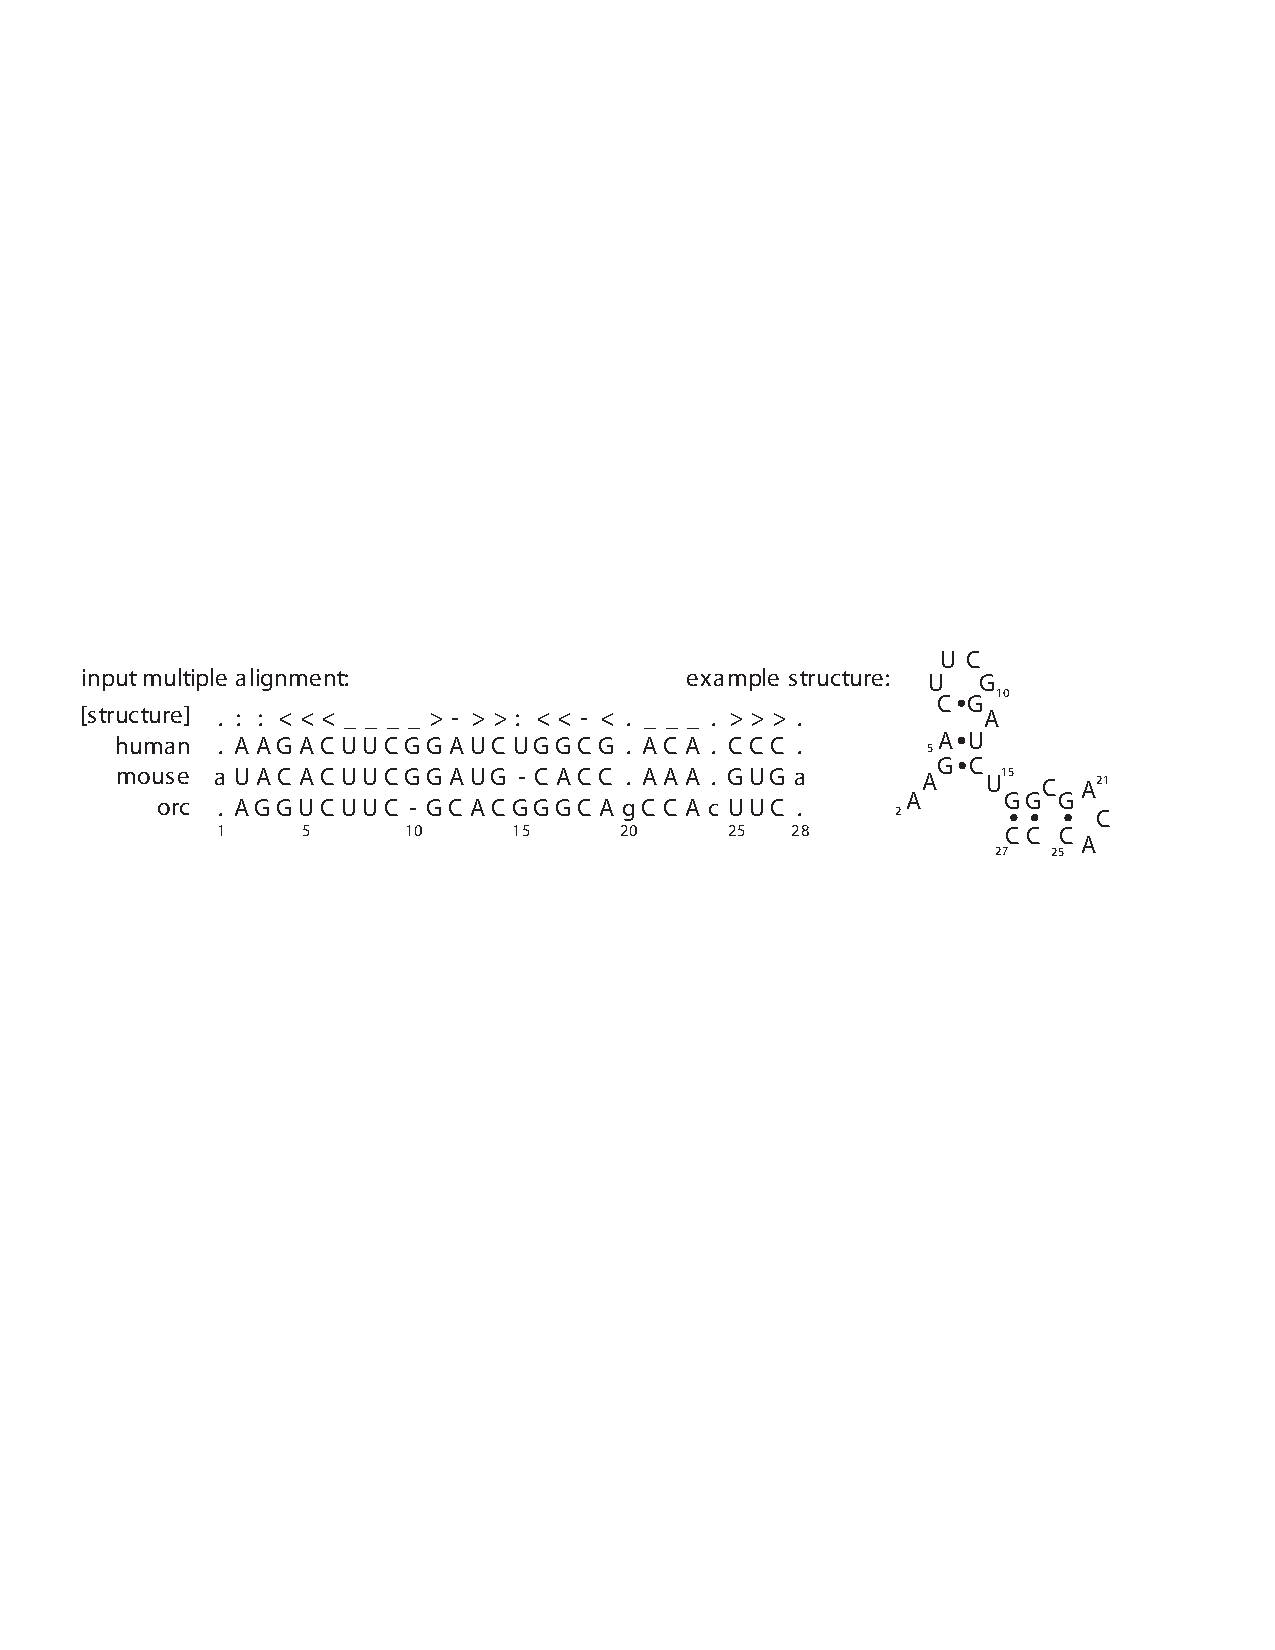
\includegraphics[width=5in]{Figures/input_alignment}
\end{center}
\caption{\textbf{An example RNA sequence family.} Top: a toy multiple
alignment of three sequences, with 28 total columns, 24 of which will
be modeled as consensus positions. The [structure] line annotates the
consensus secondary structure: $>$ and $<$ symbols mark base pairs,
$x$'s mark consensus single stranded positions, and .'s mark
``insert'' columns that will not be considered part of the consensus
model. Bottom: the secondary structure of the ``human'' sequence.} 
\label{fig:input_alignment}
\end{figure}

The guide tree has eight types of nodes:

\vspace{0.5em}
\begin{tabular}{lll}
Node      & Description      &  Production           \\ \hline
MATP  & (pair)                 & $V_{\mbox{\tiny MATP}} \rightarrow a Y b$  \\
MATL  & (single strand, left)  & $V_{\mbox{\tiny MATL}} \rightarrow a Y$   \\
MATR  & (single strand, right) & $V_{\mbox{\tiny MATR}} \rightarrow Y a$   \\
BIF   & (bifurcation)          & $V_{\mbox{\tiny BIF}}  \rightarrow
Y_{\mbox{\tiny BEGL}} Z_{\mbox{\tiny BEGR}}$ \\
ROOT  & (root)                 & $V_{\mbox{\tiny ROOT}} \rightarrow Y$       \\
BEGL  & (begin, left)          & $V_{\mbox{\tiny BEGL}} \rightarrow Y$       \\
BEGR  & (begin, left)          & $V_{\mbox{\tiny BEGR}} \rightarrow Y$       \\
END   & (end)                  & $V_{\mbox{\tiny END}}  \rightarrow \epsilon$ \\ \hline
\end{tabular}
\vspace{0.5em}
 
These node types correspond closely with a CM's final state types.
The guide tree deals with the consensus structure. For individual
sequences, we will need to deal with insertions and deletions with
respect to this consensus. The guide tree is the skeleton on which we
will organize the CM.

The input alignment is first used to construct a consensus secondary
structure (Figure~\ref{fig:cm_nodetree}) that defines which aligned
columns will be ignored as non-consensus (and later modeled as
insertions relative to the consensus), and which consensus alignment
columns are base-paired to each other.

\begin{figure}[t]
\begin{center}
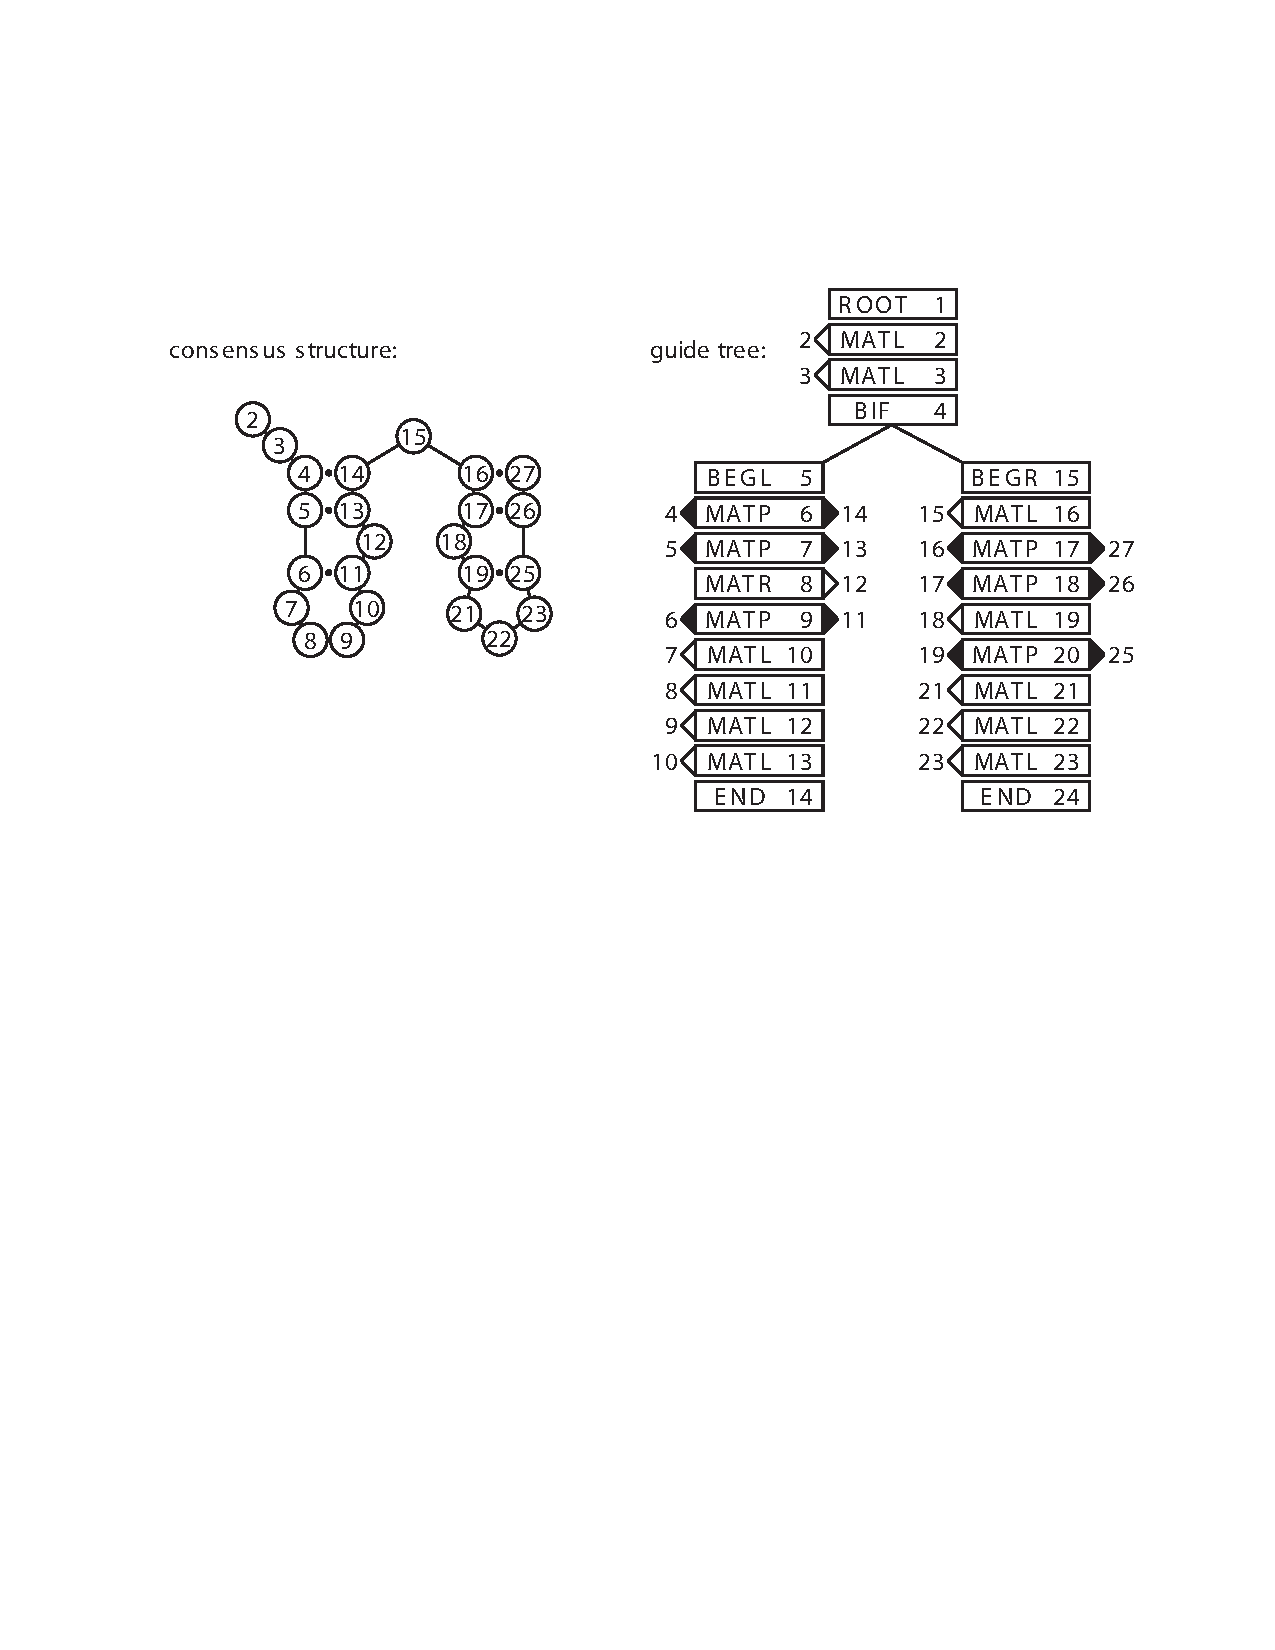
\includegraphics[width=5in]{Figures/cm_nodetree}
\end{center}
\caption{\textbf{The structural alignment is converted to a guide
tree.} Left: the consensus secondary structure is derived from the
annotated alignment in Figure~\ref{fig:input_alignment}. Numbers in
the circles indicate alignment column coordinates: e.g.  column 4 base
pairs with column 14, and so on. Right: the CM guide tree
corresponding to this consensus structure. The nodes of the tree are
numbered 1..24 in postorder traversal. MATP, MATL, and MATR nodes are
associated with the columns they generate: e.g., node 6 is a MATP
(pair) node that is associated with the base-paired columns 4 and 14.}
\label{fig:cm_nodetree}
\end{figure}

Given the consensus structure, consensus base pairs are assigned to
MATP nodes and consensus unpaired columns are assigned to MATL or MATR
nodes. One ROOT node is used at the head of the tree.  Multifurcation
loops and/or multiple stems are dealt with by assigning one or more
BIF nodes that branch to subtrees starting with BEGL or BEGR head
nodes. (ROOT, BEGL, and BEGR start nodes are labeled differently
because they will be expanded to different groups of states; this has
to do with avoiding ambiguous parse trees for individual sequences, as
will soon become apparent.) Alignment columns that are considered to
be insertions relative to the consensus structure are ignored at this
stage.

In general there will be more than one possible guide tree for any
given consensus structure. Almost all of this ambiguity is eliminated
by three conventions: (1) only MATL nodes are used for hairpin loops;
(2) in describing interior loops, MATL nodes are used before MATR
nodes; and (3) BIF nodes are only invoked where necessary to explain
branching secondary structure stems (as opposed to unnecessarily
bifurcating in single stranded sequence). One source of ambiguity
remains. In invoking a bifurcation to explain alignment columns $i..j$
by two substructures on columns $i..k$ and $k+1..j$, there may be
several possible choices of $k$ (e.g. in a single stranded region
between the two substructures). The choice of bifurcation point $k$
impacts the performance of the divide and conquer algorithm. My
current strategy is to choose $k$ such that $i..k$ and $k+1..j$ are as
close to the same length as possible.

The result of this procedure is the guide tree. The nodes of the guide
tree are numbered in post-traversal order (from root to leaves, so
parent nodes always have lower indices). The guide tree corresponding
to the input multiple alignment in Figure~\ref{fig:input_alignment} is
shown on the right in Figure~\ref{fig:cm_nodetree}.

\subsubsection{From guide tree to covariance model}

A CM must deal with insertions and deletions in individual sequences
relative to the consensus structure. For example, for a consensus base
pair, either partner may be deleted leaving a single unpaired residue,
or the pair may be entirely deleted; additionally, there may be
inserted nonconsensus residues between this pair and the next pair in
the stem. Accordingly, each node in the master tree is expanded into
one or more \emph{states} in the CM as follows:

\vspace{0.5em}
\begin{tabular}{clccc}
Node   &  States             & nstates & nsplit & ninsert \\ \hline
MATP   & [MP ML MR D] IL IR  &   6     &   4    &  2   \\
MATL   & [ML D] IL           &   3     &   2    &  1   \\
MATR   & [MR D] IR           &   3     &   2    &  1   \\
BIF    & [B]                 &   1     &   1    &  0   \\
ROOT   & [S] IL IR           &   3     &   1    &  2   \\
BEGL   & [S] IL              &   1     &   1    &  0   \\
BEGR   & [S] IL IR           &   2     &   1    &  1   \\
END    & [E]                 &   1     &   1    &  0   \\ \hline
\end{tabular}
\vspace{0.5em}

The states are grouped into a \emph{split set} of 1-4 states (shown in
brackets above) and an ``insert set'' of 0-2 insert states. The split
set includes the consensus state, which by convention is first. One
and only one of the states in the split set must be visited in every
parse tree (and this fact will be exploited by the divide and conquer
algorithm). The insert state(s) are not obligately visited, and they
have self-transitions, so they will be visited zero or more times in
any given parse tree.

State transitions are then assigned as follows. For bifurcation nodes,
the B state makes obligate transitions to the S states of the child
BEGL and BEGR nodes. Each state in a split set of a non-bifurcation
node makes a possible transition to every insert state in the
\emph{same} node, and to every state in the split set of the
\emph{next} node. An IL state makes a transition to itself, to the IR
state in the same node (if present), and to every state in the split
set of the next node. An IR state makes a transition to itself and to
every state in the split set of the next node.

This arrangement of transitions guarantees that there is unambiguously
one and only one parse tree for any given individual structure. This
is important. The algorithm will find a maximum likelihood parse tree
for a given sequence, and we wish to interpret this result as a
maximum likelihood structure, so there must be a one to one
relationship between parse trees and secondary structures
\cite{Giegerich00}.

As a convenient side effect of the ordering of the states, it is
guaranteed that the transitions from any state are to a
\emph{contiguous} set of child states, so the transitions for state
$v$ may be kept as an offset and a count; e.g. state $v$ makes
transitions to states $v+\mbox{offset}_v..v+\mbox{count}_v-1$, with offset
always $\geq 0$.  Similarly, the parent states which may transition
into $v$ are also guaranteed to be contiguous in the final CM. This
contiguity is exploited by the implementation.

Thus the final CM structure is an array of M states, connected as a
directed graph by transitions $t_v(y)$ (or probability 1 transitions
$v \rightarrow (y,z)$ for bifurcations) with the states numbered such
that $y,z \geq v$. The numbering of the states is in postorder
traversal with respect to the guide tree. There are no cycles in the
directed graph other than cycles of zero length (e.g. the
self-transitions of the insert states). This is important: since all
the transition dependencies run in one direction, we can do an
iterative dynamic programming calculation through the model states,
starting with the last numbered end state $M$ and ending in the root
state $1$.  An example CM, corresponding to the input alignment of
Figure~\ref{fig:input_alignment}, is shown in
Figure~\ref{fig:cm_graph}.

\begin{figure}[tp]
\begin{center}
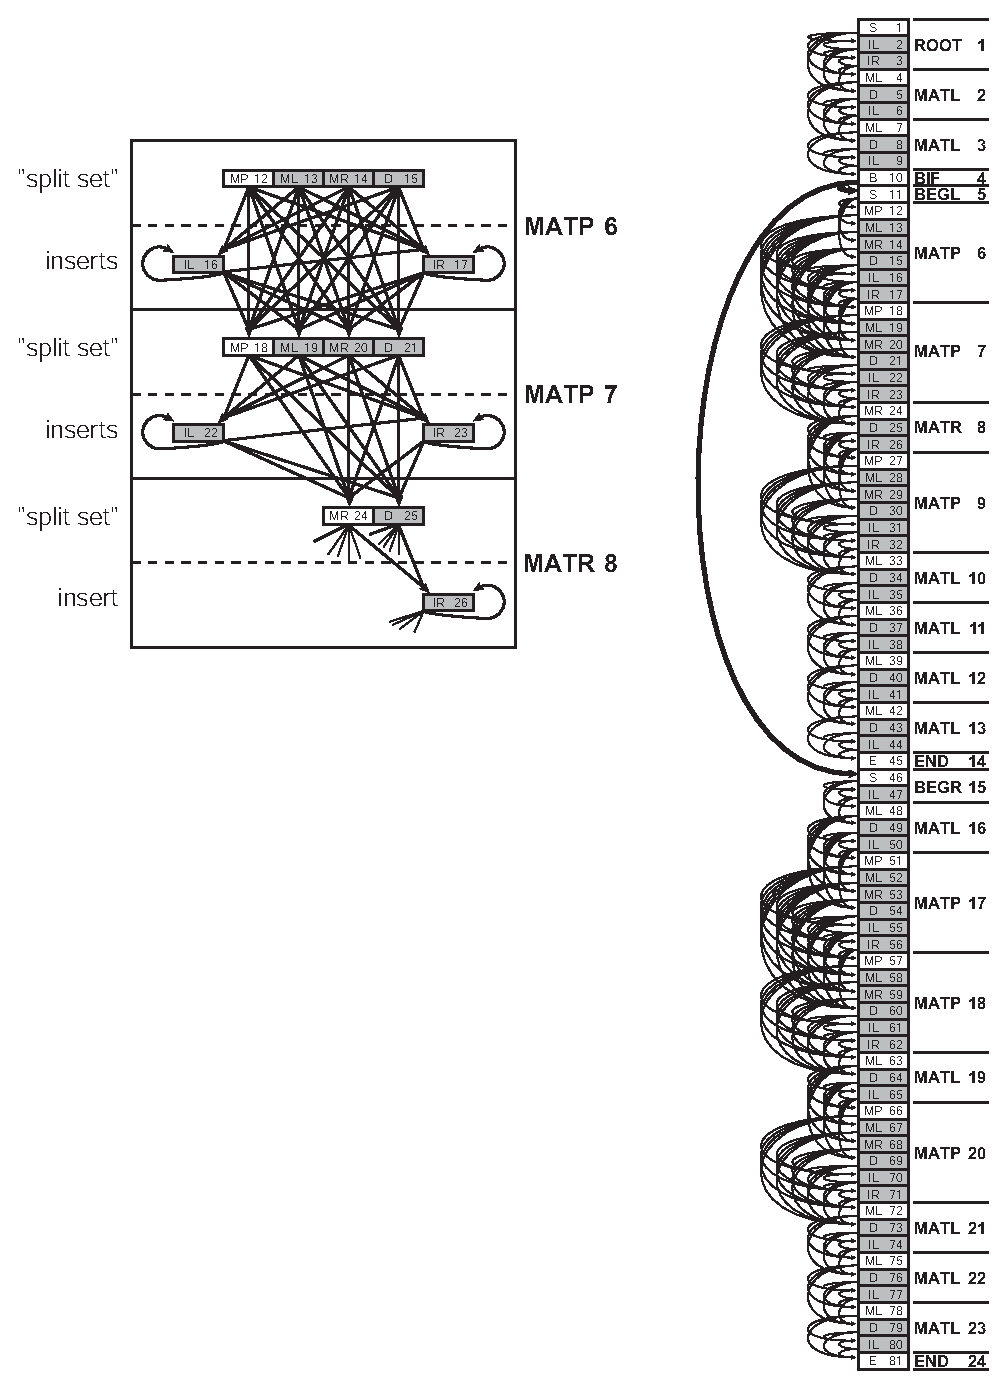
\includegraphics[width=5in]{Figures/cm_graph}
\end{center}
\caption{\textbf{A complete covariance model.} Right: the CM
corresponding to the alignment in Figure~\ref{fig:input_alignment}.
The model has 81 states (boxes, stacked in a vertical array). Each
state is associated with one of the 24 nodes of the guide tree (text
to the right of the state array). The states corresponding to the main
line of the consensus are in white. Infrequent states that are
responsible for insertions and deletions relative to consensus are
gray. The transitions from bifurcation state B10 to start states S11
and S46 are shown in bold because they are special: they are an
obligate bifurcation that happens with probability 1. All other
transitions (thin arrows) are associated with transition
probabilities.  Emission probabilities (for all but B, S, D, and E
states) are not represented in the figure. A key idea is that the
model can be thought of as an ordered array, in which all transitions
are directed to states of higher or equal index in the model. Left:
the states are also arranged according to the guide tree. A blow up of
part of the model corresponding to nodes 6, 7, and 8 is shown, to show
more clearly the logic of the connectivity of transition probabilities
(see main text), and to show how any parse tree must transit through
one and only one state in each ``split set''.}
\label{fig:cm_graph}
\end{figure}

\subsubsection{Parameterization}

Using the guide tree and the final CM, each individual sequence in the
input multiple alignment can be converted unambiguously to a CM parse
tree, as shown in Figure~\ref{fig:parsetrees}. Counts for observed
state transitions and singlet/pair emissions are then collected from
these parse trees. The observed counts are converted to transition and
emission probabilities by standard procedures (I calculate maximum a
posteriori parameters, using Dirichlet priors).

\begin{figure}[t]
\begin{center}
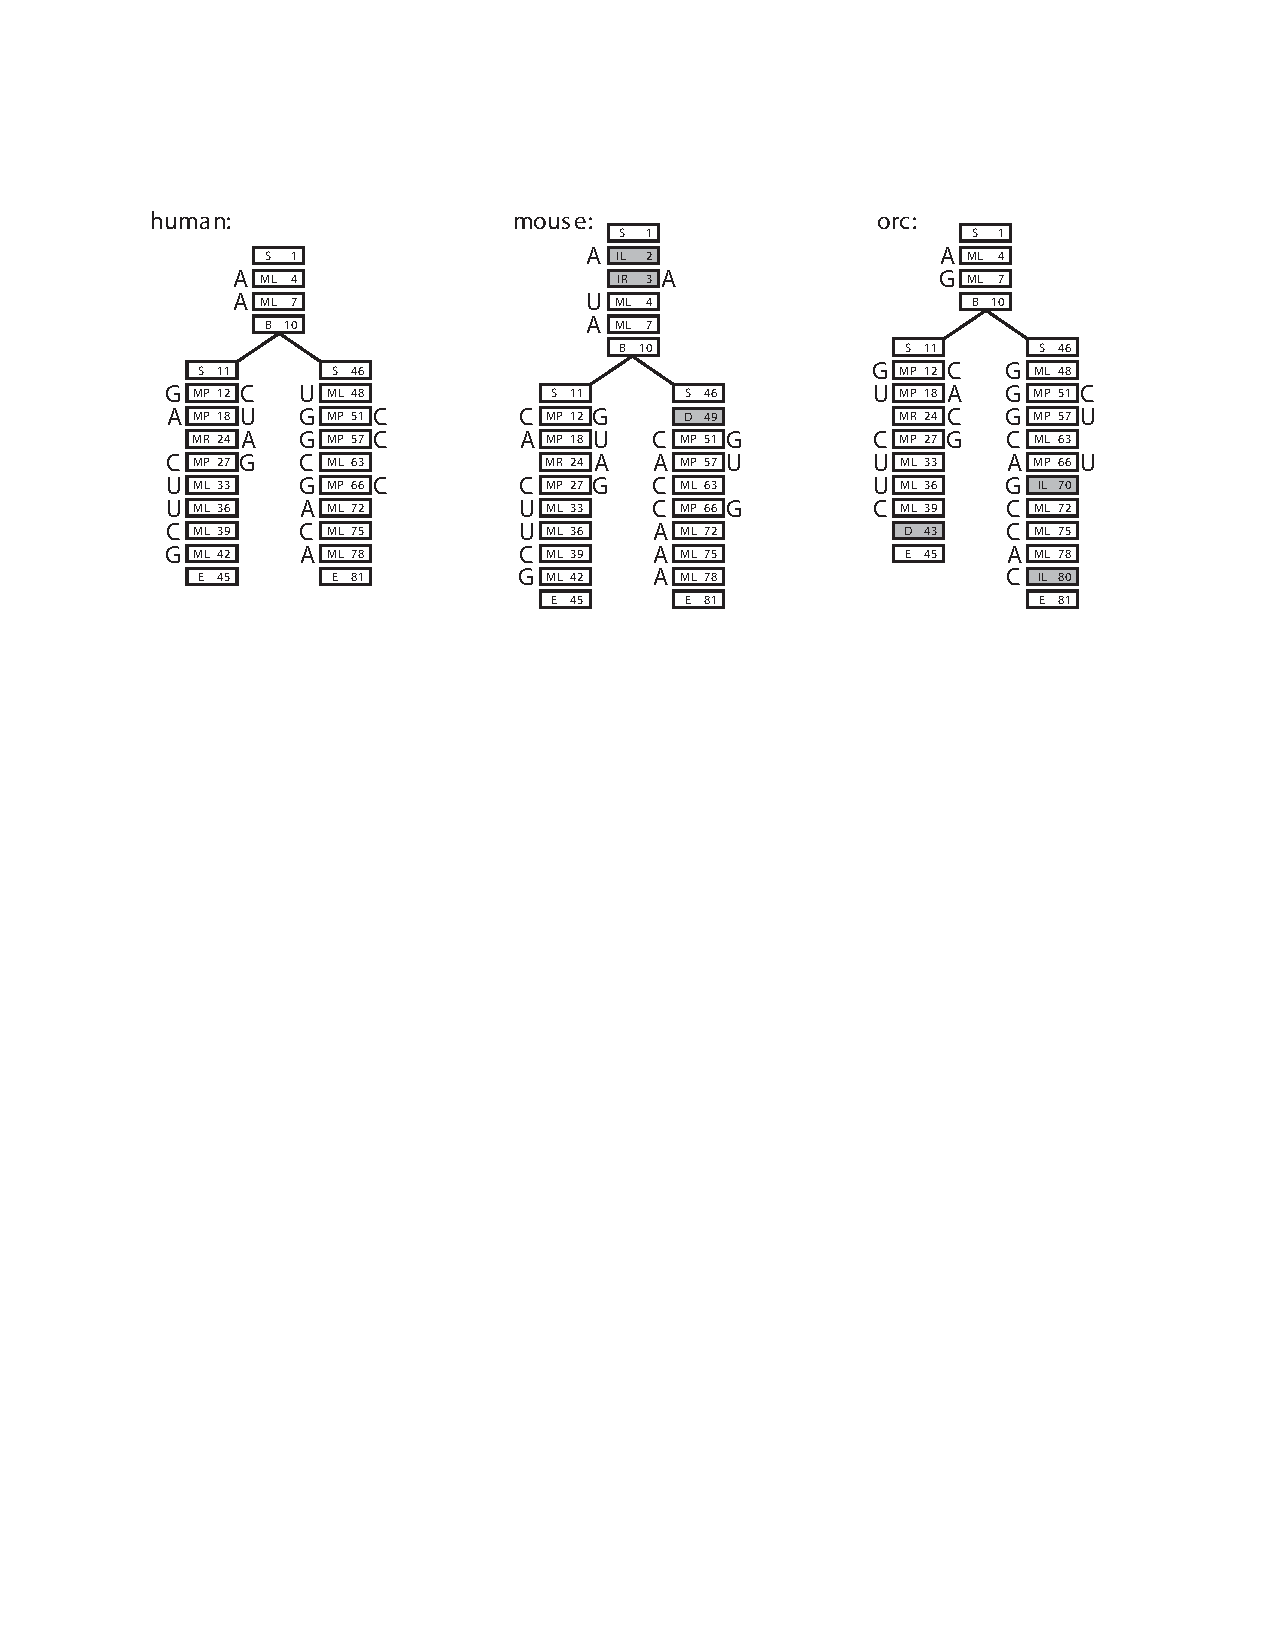
\includegraphics[width=5in]{Figures/parsetrees}
\end{center}
\caption{\textbf{Example parse trees.} Parse trees are shown for the
three sequences/structures from Figure~\ref{fig:input_alignment},
given the CM in Figure~\ref{fig:cm_graph}. For each sequence, each
residue must be associated with a state in the parse tree. (The
sequences can be read off its parse tree by starting at the upper left
and reading counterclockwise around the edge of parse tree.) Each
parse tree corresponds directly to a secondary structure -- base pairs
are pairs of residues aligned to MP states. A collection of parse
trees also corresponds to a multiple alignment, by aligning residues
that are associated with the same state -- for example, all three
trees have a residue aligned to state ML4, so these three residues
would be aligned together. Insertions and deletions relative to the
consensus use nonconsensus states, shown in gray.}
\label{fig:parsetrees}
\end{figure}

\subsubsection{Comparison to profile HMMs}

The relationship between an SCFG and a covariance model is analogous
to the relationship of hidden Markov models (HMMs) and profile HMMs
for modeling multiple sequence alignments
\cite{Krogh94,Durbin98,Eddy98}. A comparison may be instructive, at
least to readers familiar with profile HMMs.  A profile HMM is a
repetitive HMM architecture that associates each consensus column of a
multiple alignment with a single type of model node -- a MATL node, in
the above notation. Each node contains a ``match'', ``delete'', and
``insert'' HMM state -- ML, IL, and D states, in the above notation.
The profile HMM also has special begin and end states. Profile HMMs
could therefore be thought of as a special case of CMs. An
unstructured RNA multiple alignment would be modeled by a guide tree
of all MATL nodes, and converted to an unbifurcated CM that would
essentially be identical to a profile HMM. (The only difference is
trivial; the CM root node includes a IR state, whereas the start node
of a profile HMM does not.) All the other node types (especially MATP,
MATR, and BIF) and state types (e.g. MP, MR, IR, and B) are SCFG
augmentations necessary to extend profile HMMs to deal with RNA
secondary structure.


%%%%%%%%%%%%%%%%%%%%%%%%%%%%%%%%%%%%%%%%%%%%%%%%%%%%%%%%%%%%%%%%
%%%%%%%%%%%%%%%%%%%%%%%%%%%%%%%%%%%%%%%%%%%%%%%%%%%%%%%%%%%%%%%%

\subsection{Divide and conquer algorithm}

\subsubsection{Notation}

I use $v$, $w$, $y$, and $z$ as indices of states in the model. These
will range from $1..M$, for a CM with $M$ states. $S_v$ refers to the
\emph{type} of state $v$; it will be one of the nine types
\{D,P,ML,IL,MR,IL,S,E,B\}. $C_v$ is a list of children for state $v$
(states $y$ that $v$ can transit to); it will contain up to six
contiguous indices $y$ with $v <= y <= M$. $P_v$ is a list of parents
for state $v$ (states that could have transited to state $v$); it will
contain up to six contiguous indices $y$ with $1 <= y <= v$. (Because
the sets are guaranteed to be contiguous in the model, the
implementation stores these as an offset relative to $v$ and a count,
as described above.) I use $g$, $h$, $i$, $j$, $k$, $p$, and $q$ as
indices referring to positions in a sequence $x$. These indices range
from $1..L$, for a sequence of length $L$. Some algorithms will also
use $d$ to refer to a subsequence length, where $d = j-i+1$ for a
subsequence $x_i..x_j$.

The CYK/inside algorithm calculates a three-dimensional matrix of
numbers $\alpha_v(i,j)$, and CYK/outside calculates numbers
$\beta_v(i,j)$, as described below. I will refer to $v$ (states) as
\emph{deck} coordinates in the three-dimensional matrices, whereas $j$
and $i$ (sequence positions) are row and column coordinates within
each deck.  $\alpha_{v}$ and $\beta_{v}$ refer to whole
two-dimensional decks containing scores $\alpha_v(i,j)$ and
$\beta_v(i,j)$ for a particular state $v$. The dividing and conquering
will be done in the $v$ dimension, by choosing particular decks as
split points.

\subsubsection{The CYK/inside algorithm}

The CYK/inside algorithm iteratively calculates $\alpha_v(i,j)$ -- the
log probability of the most likely CM parse subtree rooted at state
$v$ that generates subsequence $x_i..x_j$ of sequence $x$. The
calculation initializes at the smallest subgraphs and subsequences
(e.g. subgraphs rooted at E states, generating subsequences of length
0), and iterates outwards to progessively longer subsequences and
larger CM subgraphs.

For example, if we're calculating $\alpha_v(i,j)$ and $v$ is a P
(pair) state, $v$ will generate the pair $x_i,x_j$ and transit to a
new state $y$ (one of its possible transitions $C_v$) which then will
have to account for the smaller subsequence $x_{i+1}..x_{j-1}$. The
log probability for a particular choice of next state $y$ is the sum
of three terms: an emission term $\log e_v(x_i,x_j)$, a transition
term $\log t_v(y)$, and an already calculated solution for the smaller
optimal parse tree rooted at $y$, $\alpha_y(i+1,j-1)$. The answer for
$\alpha_v(i,j)$ is then the maximum of all possible choices of child
states $y$ that $v$ can transit to.

The algorithm \texttt{inside} is as follows:

\begin{algorithm}
\alginout{A CM subgraph $G^r_z$ and subsequence $x_g..x_q$.}
         {Scoring matrix decks $\alpha_r..\alpha_z$.}
\algname{inside}{r,z; g,q} 
\begin{algtab*}
\algforto{$v \leftarrow z$}{$r$}
  \algforto{$j \leftarrow g-1$}{$q$} 
    \algforto{$i \leftarrow j+1$}{$g$}
       $d \leftarrow j-i+1$\\
       \algif{$S_v =$ D or S:}
       	$\alpha_v(i,j) = \max\limits_{y \in C(v)} \left[ \alpha_y(i,j)  + \log t_v(y) \right]$\\
       \algelseif{$S_v =$ P and $d>=2$:}
	$\alpha_v(i,j) = \log e(x_i, x_j) + \max\limits_{y \in C(v)} \left[ \alpha_y(i+1,j-1) + \log t_v(y) \right]$\\
       \algelseif{$S_v =$ L and $d>=1$:}
        $\alpha_v(i,j) = \log e(x_i) + \max\limits_{y \in C(v)} \left[ \alpha_y(i+1,j)   + \log t_v(y) \right]$\\
       \algelseif{$S_v =$ R and $d>=1$:}
        $\alpha_v(i,j) = \log e(x_j) +      \max\limits_{y \in C(v)} \left[ \alpha_y(i,j-1)   + \log t_v(y) \right]$ \\
       \algelseif{$S_v =$ B:}
        $(y,z) \leftarrow $ left and right S children of state $v$\\
        $\alpha_v(i,j) = \max\limits_k \left[ \alpha_y(i,k) + \alpha_z(k+1,j) \right]$ \\
       \algelseif{$S_v =$ E and $d=0$:}
	$\alpha_v(i,j) = 0$\\
       \algelse
	$\alpha_v(i,j) = -\infty$\\
\end{algtab*}
\end{algorithm}

Given a sequence $x$ of length $L$ and a CM $G$ of length $M$, we
could call \texttt{inside(1,M; 1,L)} to align the whole model (states
$1..M$) to the whole sequence ($x_1..x_L$). When \texttt{inside}
returns, $\alpha_1(1,L)$ would contain the log probability of the best
parse of the complete sequence with the complete model. 

We do not have to keep the entire $\alpha$ matrix in memory to
calculate these scores.  As we reach higher decks $\alpha_v$ in the
three dimensional dynamic programming matrix, our calculations no
longer depend on certain lower decks. A lower deck $y$ can be
deallocated whenever all the parent decks $P(y)$ that depend on it
have been calculated. \footnote{The implementation goes even further
and recycles decks when possible, saving some initialization steps and
many memory allocation calls; for example, since values in all E decks
are identical, only one E deck needs to be calculated and that
precalculated deck can be reused whenever $S_v = E$.}

This deallocation rule has a nice property that the divide and conquer
algorithm takes quiet advantage of when solving smaller subproblems
for CM subgraphs rooted at some state $w$.  When the root state $w$ is
an S state, the $\alpha$ matrix returned by \texttt{inside} contains
only one active deck $\alpha_w$. (No lower state $>w$ can be reached
from any state $<w$ without going through $w$, so all lower decks are
deallocated once deck $w$ is completed.) But when the root state $w$
is the first state in a split set $w..y$ (see below for more
explanation), all (and only) the decks $\alpha_w..\alpha_y$ are active
when \texttt{inside} returns.

In some cases we want to recover the optimal parse tree itself, not
just its score. The \texttt{inside}$^{\mathcal{T}}$ routine is a
modified version of $\texttt{inside}$. It keeps an additional ``shadow
matrix'' $\tau_v(i,j)$. A $\tau_v(i,j)$ traceback pointer either
records the index $y$ that maximized $\alpha_v(i,j)$ (for state types
D,S,MP,ML,MR,IL,IR) or records the split point $k$ that maximized
$\alpha_v(i,j)$ for a bifurcation (B) state. The $\tau$ shadow matrix
does not use the deallocation rules -- \texttt{inside}$^{\mathcal{T}}$
can only be called for problems small enough that they can be solved
within our available memory space. Thus the
\texttt{inside}$^{\mathcal{T}}$ routine works by calling
\texttt{inside} in a mode that also keeps the shadow matrix $\tau$,
and then calls a recursive traceback starting with $v,i,j$:

\begin{algorithm}
\alginout{A shadow matrix $\tau$ for CM subgraph $G^v$ rooted at state
         $v$, and subsequence $x_i..x_j$.}
         {An optimal parse tree $\mathcal{T}$.}
\algname{traceback}{v,i,j}
\begin{algtab*}
  \algif{$S_v =$ E:}
    attach $v$\\
  \algelseif{$S_v =$ S or D:}
    attach $v$ \\
    \algcall{traceback}{$\tau_v(i,j), i, j$}\\
  \algelseif{$S_v =$ P:}
    attach $x_i,v,x_j$\\
    \algcall{traceback}{$\tau_v(i,j), i+1, j-1$}\\
  \algelseif{$S_v =$ L:}
    attach $x_i,v$\\
    \algcall{traceback}{$\tau_v(i,j), i+1, j$}\\
  \algelseif{$S_v =$ R:}
    attach $v,x_j$\\
    \algcall{traceback}{$\tau_v(i,j), i,   j-1$}\\
  \algelseif{$S_v =$ B:}
    $(y,z) \leftarrow $ left and right S children of state $v$\\
    attach $v$\\
    \algcall{traceback}{$y, i, \tau_v(i,j)$}\\
    \algcall{traceback}{$z, \tau_v(i,j)+1, j$}\\
\algend
\end{algtab*}
\end{algorithm}

\subsubsection{The CYK/outside algorithm}

The CYK/outside algorithm iteratively calculates $\beta_v(i,j)$, the
log probability of the most likely CM parse tree for a CM generating a
sequence $x_1..x_L$ \emph{excluding} the optimal parse subtree rooted
at state $v$ that accounts for the subsequence $x_i..x_j$. The
calculation initializes with the entire sequence excluded (e.g.
$\beta_1(1,L) = 0$), and iterates inward to progressively shorter and
shorter excluded subsequences and smaller CM subgraphs.

A complete implementation of the CYK/outside algorithm requires first
calculating the CYK/inside numbers $\alpha$, because they are needed
to calculate $\beta_v$ when the parent of $v$ is a bifurcation
\cite{Lari90,Lari91,Durbin98}. However, the divide and conquer
algorithm only calls \texttt{outside} on unbifurcated, linear CM
subgraphs; the parent of $v$ is never a bifurcation, and the
implementation can therefore be streamlined as follows:

\begin{algorithm}
\alginout{An unbifurcated CM subgraph $G^r_z$ and subsequence $x_g..x_q$.}
         {Scoring matrix decks $\beta_r..\beta_z$.}
\algname{outside}{r,z; g,q}
\begin{algtab*}
 $\beta_v(i,j) \leftarrow -\infty \quad \forall \quad v,i,j$\\
 $\beta_r(g,q) \leftarrow 0$\\
 \algforto{$v \leftarrow r+1$}{$z$}
   \algforto{$j \leftarrow q$}{$g-1$}
     \algforto{$i \leftarrow g$}{$j+1$}
       $\beta_v(i,j) = \max\limits_{y \in P(v)} \left\{
              \begin{array}{rcl}
              \beta_y(i,j) + \log t_y(v) &:&  S_y = D,S,E \\
              \beta_y(i-1,j+1) + \log t_y(v) + \log e_y(x_{i-1}, x_{j+1}) &:& S_y = P\\
              \beta_y(i-1,j) + \log t_y(v) + \log e_y(x_{i-1}) &:& S_y = L\\
              \beta_y(i,j-1) + \log t_y(v) + \log e_y(x_{j+1})  &:& S_y = R \\
              \end{array} \right.$
\end{algtab*}
\end{algorithm}

As with \texttt{inside}, we do not keep the entire $\beta$ matrix in
memory. A deck $\beta_v$ can be deallocated when all child decks
$C(v)$ that depend on the values in $\beta_v$ have been
calculated. This means that if the last deck $z$ is a bifurcation or
end state, $\beta_z$ will be the only active allocated deck when
\texttt{outside} returns. If $z$ is the last state in a split set
$w..z$, all (and only) the split set decks $\beta_w..\beta_z$ will be
active when \texttt{outside} returns.

\subsubsection{Using CYK/inside and CYK/outside to divide and conquer}

Now, for any chosen state $v$, $\argmax\nolimits_{i,j} \alpha_{v}(i,j) +
\beta_{v}(i,j)$ tells us which cell $v,i,j$ the optimal parse tree
passes through, conditional on using state $v$ in the parse. We know
that any parse tree must include all the bifurcation and start states
of the CM, so we know that the optimal alignment \emph{must} use any
chosen bifurcation state $v$ and its child start states $w$ and
$y$. Thus, we are guaranteed that:

\[
   \max_{i,k,j} \beta_{v}(i,j) + \alpha_{w}(i,k) + \alpha_{y}(k+1,j)
\]

is the optimal overall alignment score, and we also know that

\[
      (i,k,j) = \argmax_{i',k',j'}  \beta_{v}(i',j') +
      \alpha_{w}(i',k') + \alpha_{y}(k'+1,j') 
\]

gives us a triplet that identifies three cells that must be in the
optimal alignment -- $(v,i,j)$, $(w,i,k)$, and $(y,k+1,j)$. This
splits the remaining problem into three smaller subproblems -- an
alignment of the sequence $x_{i}..x_{k}$ to a CM subgraph $w..y-1$, an
alignment of the sequence $x_{k+1}..x_{j}$ to a CM subgraph $y..M$,
and an alignment of the two-piece sequence
$x_1..x_{i-1}//x_{j+1}..x_L$ to a CM subgraph $1..v$.

The subproblems are then themselves split, and this splitting can
continue recursively until all the bifurcation triplets on the optimal
parsetree have been determined.

At this point the remaining alignment subproblems might be small
enough to be solved by straightforward application of the standard
CYK/inside algorithm (e.g. \texttt{inside}$^\mathcal{T}$). However,
this is not guaranteed to be the case. A second division strategy is
needed that does not depend on splitting at bifurcations.

For the second strategy, we take advantage of the fact that we know
that the optimal parse tree must also include one and only one state
from the split set of each node (e.g. the non-insert states in the
node). Let $w..y$ be the indices of a split set of states in the
middle of the current model subgraph. ($w..y$ can be at most 4
states.)  We know that

\[
(v,i,j) = \argmax_{v' \in w..y,i',j'} \alpha_{v'}(i',j') + \beta_{v'}(i',j')
\]

gives us a new cell $(v,i,j)$ in the optimal parse tree, and splits
the problem into two smaller problems. This strategy can be applied
recursively all the way down to single nodes, if necessary. We can
therefore guarantee that we will never need to carry out a full
CYK/inside alignment algorithm on any subproblem. The most
memory-intensive alignment problem that needs to be solved is the very
first split.  The properties of the first split determine the memory
complexity of the algorithm.

If we look at the consequences of these splitting strategies, we see
we will have to deal with three types of problems
(Figure~\ref{fig:splitter_schematic}):

\begin{itemize}
\item A \emph{generic problem} means finding the optimal alignment of
a CM subgraph $G_{r..z}$ to a contiguous subsequence $x_g..x_q$. The
subgraph $G_{r..z}$ corresponds to a complete subtree of the CM's
guide tree -- e.g. state $r$ is a start (S), and state $z$ is an end
(E). $G_{r..z}$ may contain bifurcations. The problem is solved in one
of two ways. If $G_{r..z}$ contains no bifurcations, it is solved as a
wedge problem (see below). Else, the problem is subdivided by the
bifurcation-dependent strategy; an optimal triple $(i,k,j)$ is found
for a bifurcation state $v$ and its children $w,y$, splitting the
problem into a V problem and two generic problems.

\item A \emph{wedge problem} means finding the optimal alignment of an
unbifurcated CM subgraph $G_{r..z}$ to a contiguous subsequence
$x_g..x_q$. State $r$ does not have to be a start state (S); it may be
a state in a split set (MP, ML, MR, or D). State $z$ is an end (E).  A
wedge problem is solved by the split set-dependent strategy: an
optimal $(v,i,j)$ is found, splitting the problem into a V problem and
a smaller wedge problem.

\item A \emph{V problem} consists of finding the optimal alignment of
an unbifurcated CM subgraph $G_{r..z}$ to a noncontiguous, two-piece
sequence $x_g..x_h//x_p..x_q$, exclusive of the residues $x_h$ and
$x_p$ (open circles in Figure~\ref{fig:splitter_schematic}).  State
$r$ can be a start state or any state in a split set; the same is true
for $z$. A V problem is solved by a split set-dependent strategy: an
optimal $(v,i,j)$ is found, splitting the problem into two V problems.
\end{itemize}

\begin{figure}
\begin{center}
\includegraphics[width=5in]{Figures/splitter_schematic}
\end{center}
\caption{\textbf{The three types of problems that need to be split.}
The sequence axis (e.g. $x_g..x_q$) is horizontal. The model subgraph
axis for a contiguous set of states (e.g. states $r..z$) is vertical.
Closed circles indicate ``inclusive of'', and open circles indicate
``exclusive of''.}
\label{fig:splitter_schematic}
\end{figure}

The three recursive splitting algorithms to solve these problems
are as follows:

\subsubsection{The generic\_splitter routine}
\begin{algorithm}
\alginout{A generic problem, for CM subgraph $G_{r..z}$ and
          subsequence $x_{g..q}$.}
         {An optimal parse subtree $\mathcal{T}$.}

\algname{generic\_splitter}{r,z; g,q}
\begin{algtab*}
\algif{alignment problem is small:}
  \algreturn \algcall{inside$^\mathcal{T}$}{r,z; g,q}\\
\algelseif{no bifurcation in $G_{r..z}$:}
  \algreturn \algcall{wedge\_splitter}{r,z; g,q}\\
\algelse
   $v   \leftarrow$ lowest numbered bifurcation state in subgraph $G_{r..z}$.\\
   $w,y \leftarrow$ left and right S children of $v$.\\
   $\beta_v \leftarrow$  \algcall{outside}{r,w; g,q}\\
   $\alpha_w \leftarrow$ \algcall{inside}{w,y-1; g,q}\\
   $\alpha_y \leftarrow$ \algcall{inside}{y,z; g,q}\\

   $(i,k,j) \leftarrow \argmax_{i',k',j'} \alpha_w(i',k') + \alpha_y(k'+1,j') + \beta_v(i',j')$ \\

   $\mathcal{T}_1   \leftarrow$ \algcall{V\_splitter}{r,v; g,i; j,q}\\
   $\mathcal{T}_2 \leftarrow$ \algcall{generic\_splitter}{w,y-1; i,k}\\
   $\mathcal{T}_3 \leftarrow$ \algcall{generic\_splitter}{y,z; k+1,j}\\

   Attach S state $w$ of $\mathcal{T}_2$ as left child of B state $v$ in $\mathcal{T}_1$.\\
   Attach S state $y$ of $\mathcal{T}_3$ as right child of B state $v$ in $\mathcal{T}_2$.\\
  
   \algreturn $\mathcal{T}_1$.\\
\algend
\end{algtab*}
\end{algorithm}

\subsubsection{The wedge\_splitter routine}
\begin{algorithm}
\alginout{A wedge problem, for unbifurcated CM subgraph $G_{r..z}$ and
          subsequence $x_{g..q}$.}
         {An optimal parse subtree $\mathcal{T}$.}

\algname{wedge\_splitter}{r,z; g,q}
\begin{algtab*}
\algif{alignment problem is small:}
  \algreturn \algcall{inside$^\mathcal{T}$}{r,z; g,q}\\
\algelse
  $(w..y) \leftarrow$ a split set chosen from middle of $G_{r..z}$\\
  $(\alpha_w..\alpha_y) \leftarrow$ \algcall{inside}{w,z; g,q}\\
  $(\beta_w..\beta_y)   \leftarrow$ \algcall{outside}{r,y; g,q}\\
  $(v,i,j) \leftarrow \argmax\limits_{v',i',j'} 
	\alpha_{v'}(i',j') + \beta_{v'}(i',j')$\\
  $\mathcal{T}_1 \leftarrow$ \algcall{V\_splitter}{r,v; g,i; j,q}\\
  $\mathcal{T}_2 \leftarrow$ \algcall{wedge\_splitter}{v,z; i,j}\\
  Attach $\mathcal{T}_2$ to $\mathcal{T}_1$ by merging at state $v$.\\
  
  \algreturn $\mathcal{T}_1$.\\
\algend
\end{algtab*}
\end{algorithm}

\subsubsection{The V\_splitter routine}
\begin{algorithm}
\alginout{A V problem, for unbifurcated CM subgraph $G_{r..z}$ and
          two-part subsequence $x_{g..h}//x_{p..q}$.}
         {An optimal parse subtree $\mathcal{T}$.}

\algname{V\_splitter}{r,z; g,h; p,q}
\begin{algtab*}
\algif{alignment problem is small:}
  \algreturn \algcall{vinside$^\mathcal{T}$}{r,z; g,h; p,q}\\
\algelse
  $(w..y) \leftarrow$ a split set chosen from middle of $G_{r..z}$\\
  $(\alpha_w..\alpha_y) \leftarrow$ \algcall{vinside}{w,z; g,h; p,q}\\
  $(\beta_w..\beta_y)   \leftarrow$ \algcall{voutside}{r,y; g,h; p,q}\\
  $(v,i,j) \leftarrow \argmax_{v'=w..y, i'=g..h, j'=p..q} 
	\alpha_{v'}(i',j') + \beta_{v'}(i',j')$\\
  $\mathcal{T}_1 \leftarrow$ \algcall{V\_splitter}{r,v; g,i; j,q}\\
  $\mathcal{T}_2 \leftarrow$ \algcall{V\_splitter}{v,z; i,h; p,j}\\
  Attach $\mathcal{T}_2$ to $\mathcal{T}_1$ by merging at state $v$.\\
  \algreturn $\mathcal{T}_1$.\\
\algend
\end{algtab*}
\end{algorithm}

\subsubsection{The vinside and voutside routines}

The \texttt{vinside} and \texttt{voutside} routines are just
\texttt{inside} and \texttt{outside}, modified to deal with a
two-piece subsequence $x_g..x_h//x_p..x_q$ instead of a contiguous
sequence $x_g..x_q$. These modifications are fairly obvious.  Most
obviously, the range of $i,j$ is restricted so that $i<=h$ and $j>=p$.
Also, \texttt{vinside(w,z; g,h; p,q)} initializes $\alpha_z(h,p) = 0$:
that is, we know that sequence $x_h..x_p$ has already been accounted
for by a CM parse tree rooted at $z$. 

\subsubsection{Implementation}

In the description of the algorithms above, some technical detail has
been omitted - in particular, a detailed description of efficient
initialization steps, and details of how the matrix coordinates can be
transformed for more highly optimized memory usage. (\texttt{inside}
and \texttt{outside} are actually implemented in a so-called $v,j,d$
coordinate system, where $d = j-i+1$ is the length of the subsequence
$x_i..x_j$; \texttt{vinside} and \texttt{voutside} are implemented in
a so-called $v,j,i$ coordinate system.) 

These details are not necessary for a high level understanding of the
divide and conquer algorithm. However, they may be necessary for
reproducing a working implementation. Extensively commented ANSI/C
source code for a reference implementation is therefore freely
available at \url{http://www.genetics.wustl.edu/eddy/infernal/} under
a GNU General Public License. This code has been tested on GNU/Linux
platforms.

In this codebase, the CM data structure is defined in
\texttt{structs.h}. The CM construction procedure is in
\texttt{modelmaker.c:Handmodelmaker()}. The guide tree is constructed
in \texttt{HandModelmaker()}. A CM is constructed from the guide tree
by \texttt{cm\_from\_master()}. Individual parse trees are constructed
using the guide tree by \texttt{transmogrify()}.

The divide and conquer algorithm is implemented in
\texttt{smallcyk.c:CYKDivideAndConquer()}, which will recursively call
a set of functions: the three splitting routines
\texttt{generic\_splitter()}, \texttt{wedge\_splitter()}, and
\texttt{V\_splitter}; the four alignment engines \texttt{inside()},
\texttt{outside()}, \texttt{vinside()}, and \texttt{voutside()}; and
the two traceback routines \texttt{insideT()} and \texttt{vinsideT()}.


%%%%%%%%%%%%%%%%%%%%%%%%%%%%%%%%%%%%%%%%%%%%%%%%%%%%%%%%%%%%%%%%
%%%%%%%%%%%%%%%%%%%%%%%%%%%%%%%%%%%%%%%%%%%%%%%%%%%%%%%%%%%%%%%%


\begin{tabular}{lrrrrrr}
                      & tRNA  & 5S rRNA  & SRP RNA & RNase P & SSU rRNA & LSU rRNA \\\hline
consensus columns     &   72  &    116   &    301  &    379  &   1545   &    2898\\
CM states ($M$)       &  230  &    357   &    927  &   1176  &   4789   &    9023\\
base pairs (MATP)     &   21  &     35   &     89  &    113  &    462   &     794\\
unpaired (MATL$+$MATR)&   30  &     46   &    123  &    153  &    621   &    1310\\
bifurcations ($M_B$)  &    2  &      1   &      4  &      7  &     30   &      65\\
Maximum decks needed  &   13  &     12   &     13  &     13  &     18   &      20\\
Sequence length ($N$) &   73  &    120   &    300  &    377  &   1542   &    2904\\
Full CYK RAM, MB      &  2.6  &   10.7   &  168.9  &  336.7  &22705.0   &151349.7\\
Divide \& conquer RAM &  0.2  &    0.4   &    2.4  &    3.7  &   85.9   &   337.9\\
Full CYK CPU time, sec&  0.2  &    0.7   &   12.6  &   28.1  &    n.d.  &    n.d.\\
Divide \& conquer time&  0.2  &    0.9   &   22.7  &   36.8  & 3688.5   & 32089.6\\\hline
\end{tabular}



\bibliography{distilled}









\end{document}



